\documentclass{article}
\usepackage[french]{babel}
\usepackage[T1]{fontenc}

\usepackage{graphicx} % Required for inserting images
\graphicspath{{C:/Users/chabe/Documents/L3/PROJET/Projet/CRFinal/ressources/}}
\usepackage{amsmath}
\usepackage{amsfonts}
\usepackage{fancyhdr}
\usepackage{csquotes}
\usepackage{biblatex}
\addbibresource{Attracteur de Lorenz.bib}

\usepackage{thmbox}

\usepackage{tikz}
\usepackage[firstpage = True]{background}
\usepackage{wrapfig}



\pagestyle{fancy}
\fancyhead{}
\fancyfoot{}
\fancyhead[L]{Attracteur de Lorenz - \thesection}
\fancyhead[R]{
\includegraphics[height =15pt]{logoUPS}}
\setlength{\headheight}{20pt}
\fancyfoot[C]{\thepage}

\title{Système de Lorenz}


\newcommand*\colv[1]{
\left(\begin{array}{c}
    #1
\end{array}\right)
}

\newcommand{\R}{\mathbb{R}}

\newcommand{\deriv}[3][ ]{
    \ensuremath{\frac{\mathrm{d}^{#1}#2}{\mathrm{d}^{#1} #3}}
}
\newcommand{\id}[1][]{\ensuremath{\mathrm{Id}_{#1}}}

\newcommand{\cad}{c'est-\`a-dire }

\newcommand{\setbackground}[1]{ \backgroundsetup{ scale=1, opacity=1, angle=0, contents={ \includegraphics[width=\paperwidth]{#1} } } }

\newtheorem[M , nocut]{prop}{Proposition}[section]
\newtheorem[M]{propt}{Propriété}[section]
\newtheorem[L , nocut]{thm}{Théoreme}
\newtheorem[L]{cor}{Corollaire}

\begin{document}
\begin{titlepage}
    \BgThispage
    \setbackground{LorenzTransparentbis}
    \clearpage
    \begin{center}
        \vspace{1cm} 
        \Huge
        \textbf{Attracteur de Lorenz}\\
        \vspace{0.5cm}
        \Large
        Projet de licence 3\\
        \vspace{1.5cm}
            
        \textbf{Adrien CHABERT\\Louka OUKALA\\Salome COUDIERE}    
        \vfill
        Second semestre - Année 2023-2024
    \end{center}
\end{titlepage}

\tableofcontents
\thispagestyle{empty}
\newpage

\section*{Introduction}
\thispagestyle{empty}
\setcounter{page}{1}
\begin{quotation}
    Does a flap of a butterfly's wings in Brazil set off a tornado in Texas?
\end{quotation}
C'est le titre de l'article que Edward N. Lorenz publie en 1972 \cite{lorenz_does_1972}, dans lesquels il fais la synthèse de ce que l'on connait sous le nom de la théorie du chaos. La question peut être traduite par "Es-ce qu'un battement d'ailes de papillon peut entrainer une tornade au Brésil ?". En effet lors de l'étude de certains systèmes une faible variation peut entrainer des changements considérable dans les états ultérieurs du système. Tout au long de sa vie Lorenz ce seras intéressé au systèmes chaotiques essentiellement appliqué a son domaine de recherche : la météorologie. Dès 1963 il propose un modèle simplifié pour essayer de décrire la méteo \cite{lorenz1963}. Cependant les simplifications étant trop restrictives il est assez rare d'observer les comportement décris par ces équations dans la nature. Nous nous interresseront uniquement à l'étude mathématique de ce système. Ce système est appellé l'attracteur de Lorenz (aussi appellé attracteur étrange ou système de Lorenz).
\begin{equation}
    \label{Lorenz}
    \left\{
    \begin{array}{rl}
        x' &=\sigma(y-x) \\
        y' &=\rho x -y - xz\\
        z' &=xy - \beta z
    \end{array}
    \right.
    \begin{array}{r}
        (L_1)\\
        (L_2)\\
        (L_3)
    \end{array}
\end{equation}
(\textit{avec $\sigma,\rho,\beta$ des paramètres}).
A travers cette études nous allons présenter certaines caractéristique chaotiques du système en modélisant les résultats théorie avec des applications numérique, nous pourront notament observer les courbes qui prennent la forme d'ailes de papillon qui donneront leur nom a l'effet eponyme.
   
    \newpage
\section{Méthodes numériques}

Dans cette section nous allons introuire les méthodes numérique pour la résolution d'équation differentielle ordinaires (EDO). 
\begin{example}[Problématique]
    Pourquoi introduire des méthodes numériques pour la résolution des EDO ? 
\end{example}
Lorsque on étudie des équations differentielles la théorie nous permet sous certaines condition d'affirmer que la solution à un problème de Cauchy existe et est maximale. Cependant leur expressions explicite n'est pas garantie par exemple pour les EDO linéaire a coefficients constant il est systématiquement possible de trouver une solution analytique. Cependant lorsque on aborde les EDO non-linéaire, la plupart du temps nous ne sommes pas capable d'expliciter la solution analytique. C'est pourquoi on introduit les métodes numériques.\\
Commençons par introduire la forme générale d'une équation différentielle\footnote{NB: Ici on présente les méthode numériques dans $\R^3$ on peut se ramener au cas d'un espace métrique plus général}.
\[
    u'(t) = f(t,u(t)),\quad \text{avec } f\in C^1(]a,b[ \times \R^3 ;\R^3)\text{ et }u : \R^3 \to \R^3
\]
Ici $u$ est la fonction à déterminer. Alors d'après le théoreme de Cauchy-Lipschitz il existe une solution maximale et $C^1$ au problème de Cauchy suivant sur l'intervalle $[t_I,t_F] \subset ]a,b[ $:
\[
    \left\{\begin{array}{l}
        u'(t)=f(t,u)\\
        u(t_I) = \nu
    \end{array}\right.
\]
Maintenant que nous savons que la solution existe sur un intervalle de temps fermé , on cherche a approcher les valeurs de la solutions numériquement. Pour cela, on subdivise l'intervalle $[t_I,t_F]$ en $N$ sous intervalles et on calcule a l'aide d'un schéma numérique donné, la valeur approché de la solution pour tout les temps $t_n,\ 0\le n \le N$

\subsection*{Première méthode numérique, le schéma d'Euler explicite}
On introduit maintenant la première méthode de résolution.
\begin{thm}
    On note $(y_n)_{0 \le n \le N}$ la suite des approximation des valeurs de $u$ aux points $(t_n)_{0 \le n \le N}$. On appelle $h$ le pas de la méthode, et $h:= \frac{t_F-t_I}{N}$. Alors on a:
    \[
        \left\{\begin{array}{rcl}
        t_n &=& t_0 + n h \\
        y_{n+1} &=& y_n + h f(t_n,y_n)\\
        y_0 &=& \nu
        \end{array}\right. \forall 0 \le n \le N
    \]
\end{thm}
\begin{proof}
    On intègre notre équation differentielle entre les instants $t_{n}$ et $t_{n+1}$, il vient:
    \[
      u(t_{n+1}) - u(t_n) = \int_{t_n}^{t_{n+1}} f(x,u(x))\ \mathrm{d}x
    \]
    On approche l'intégrale par la méthode des rectangles et on obtient:
    \[
        \int_{t_n}^{t_{n+1}} f(x,u(x))\ \mathrm{d}x = (t_{n+1}-y_n)f(t_n,u(t_n))
    \]Or $\forall n , u(t_n) \approx y_n $, d'où:
    \[
        y_{n+1} = y_n + h f(t_n,y_n)
    \]De plus $u(t_0) = \nu = y_0$. On obtient alors le schéma d'Euler explicite.
\end{proof}
Le schéma d'Euler est une méthode simple à utiliser et à implémenter. Cependant l'ordre de son érreur, en effet la métode de Euler est d'ordre 2 (\cad que l'érreur décroit comme une une droite de pente 2 a l'échelle logarithmique selon le nombre de subdivision de notre intervalle de départ). 
\subsection*{Le schéma de Runge-Kutta}
On s'interresse maintenant au schémas de Runge-Kutta ces schémas sont des méthodes dites multi-pas (\cad on fait une moyenne pondéré de l'approximation en plusieurs point). Plus particulièrement, la méthode de Runge-Kutta 4.
\begin{thm}
    On approche les valeurs de la solution de l'équation differentielle par la suite $(y_n)_{0\le n \le N}$ sur l'intervalle $[t_I,t_F]$, avec $N$ le nombre de subdivision de l'intervalle. Alors on a: 
    \begin{align*}
    k_1 &= h f(t_n, y_n) \\
    k_2 &= h f\left(t_n + \frac{h}{2}, y_n + \frac{1}{2}k_1\right) \\
    k_3 &= h f\left(t_n + \frac{h}{2}, y_n + \frac{1}{2}k_2\right) \\
    k_4 &= h f(t_n + h, y_n + k_3)\\
    y_{n+1} &= y_n + \frac{1}{6}(k_1 + 2k_2 + 2k_3 + k_4) 
    \end{align*}
    La méthode de Runge-Kutta 4 est d'ordre 4.
\end{thm}
On admet la démonstration de cette méthode. Aussi on la choisira pour illustrer les résultats sur le système de Lorenz. Les paramètre que nous utiliserons sont les suivants, $[t_I,t_F] = [0,30], h = 0.01 \text{ et }u(t=0)= (6,4,2)$
\vfill

\section{Existence et première propriété}

Dans cette section nous allons faire une étude du systeme de Lorenz afin de determiner l'existence des solutions. Nous nous limiterons à l'étude des temps positifs ($t \ge 0$). Pour cela on transforme l'équation \eqref{Lorenz} sous une forme plus pratique pour l'étude on a alors:
\begin{equation}
    \label{fLorenz}
    \deriv{\Vec{u}}{t} = \Gamma(\Vec{u}), \quad
    \Gamma : \Vec{u} = \colv{x\\y\\z} \in \R^3 \mapsto \colv{\sigma(y-x) \\ \rho x-y-xz \\ xy-\beta z}
    \end{equation}
Commençons notre étude du système.
\begin{prop}
    Le systeme de Lorenz admet des solutions. De plus les solutions sont globales sur $\R_+$ et de classe $C^1$
\end{prop}

\begin{proof}
    $\Gamma$ est $C^1$ donc elle est localement Lipschitzienne, de plus elle de depend pas directement du temps. D'après le théoreme de Cauchy-Lipschitz, l'équation \eqref{Lorenz} admet une unique solution maximale de classe $C^1$ que l'on notera $(I,(x,y,z))$ avec $I \subset \R_+$ avec $I = [0,T[,\ T \in ]0,+\infty]$. Montrons que $(I,(x,y,z))$ est globale. Dans \eqref{Lorenz} on s'intéresse à la somme de, $x$ fois première ligne avec $y$ fois la seconde ligne et $z$ fois la troisième ligne.
\[
    xx'+yy'+zz' = \sigma yx - \sigma x^2 + \rho xy - y^2 -xyz + xyz - \beta z^2\\
\]  
Posons $\mathcal{N}: (t) \in \R^3 \mapsto x(t)^2 + y(t)^2 + z(t)^2$ ($\mathcal{N}$ est la norme euclidienne au carré)

\begin{align*}
    \Rightarrow \frac{1}{2}\deriv{ }{t}\mathcal{N}(t) & =(\sigma + \rho)x(t)y (t) -\sigma x^2(t) - y^2(t) - \beta z^2(t)\\
    & \le (\sigma + \rho)x(t)y(t) +\min (1,\sigma,\beta)\mathcal{N}(t)\\
    & \le (\frac{\sigma+\rho}{2})(x^2(t) + y^2(t)) +\min (1,\sigma,\beta) \mathcal{N}(t) &&\mathit{(Young)}\footnotemark \\
    & \le (\frac{\sigma+\rho}{2})(x^2(t) + y^2(t) + z^2(t)) +\min (1,\sigma,\beta) \mathcal{N}(t)\\
    & \le \bigg[\frac{\sigma + \rho}{2} + \min (1,\sigma,\beta) \bigg] \mathcal{N}(t)
\end{align*}
\footnotetext{$\forall p,q \in \mathbb{N}\: \text{tels que} \frac{1}{p}+\frac{1}{q}=1 \Rightarrow \forall a,b \in \R \: ab \le \frac{a^p}{p}+\frac{b^q}{q}$}

Posons $ \eta = \sigma + \rho - 2 \min (1,\sigma,\beta)$. On a alors: 
\[
    \forall t \in \R_+, \  \deriv{}{t}\mathcal{N}(t) \le \eta\  \mathcal{N}(t)
\]
D'après le lemme de Grönwall il vient:
\[
    \forall t \in \R_+,\  \mathcal{N}(t) \le \mathcal{N}_0 e^{\eta t},\  \textrm{avec } \mathcal{N}_0 = \mathcal{N}(0)
\]
Donc la norme du vecteur solution n'explose pas en temps fini.
\end{proof}

En ayant obtenue les résultats de la proposition on peut aisément en déduire que la propriété suivante.

\begin{propt}
    Les solutions du système de Lorenz \eqref{Lorenz} sont de classe $C^\infty$
\end{propt}

\begin{proof}
    Par \eqref{fLorenz} on a que $(x',y',z') = \Gamma(x,y,z)$, or par composition $\Gamma(x,y,z)$ est $C^1$ donc $(x',y',z')$ l'est aussi, ainsi $(x,y,z)$ est $C^2$.De la même manière on obtient par récurence immédiate que $(x,y,z)$ est $C^\infty$
\end{proof}

Cette propriété nous permet de dire que même si \eqref{Lorenz} est un système dit chaotique, on peut affirmer que les solutions sont régulière.

\section{\'Etude des points stationnaires}
Après une première etude sommaire du système de Lorenz \eqref{Lorenz}, on s'intéresse maintenant à l'étude des points stationnaires. Les points stationnaires sont des points tels que si le système passe par un de ces points il y reste indéfiniment.

%vérifier la formulation de ce théoreme
\begin{thm}
    Soit l'équation differentielle bien définie,
    \begin{equation*}
        u'=f(u)
    \end{equation*}
    Si il existe $v$ tel que $f(v)=0$ alors $v$ est un point stationnaire de l'équation differentielle.
\end{thm}

\subsection{Rappel des théorèmes}
\label{sec:Rappel-des-théorèmes}
D'abord on rappelle les résultats sur lesquels on s'appuiras dans la suite. Ces théorèmes établissent des résultats de stabilité sur les point stationnaires en se basant sur l'étude spectrale de la différentielle.
\begin{thm}
    \label{thm:eq-ass-stable}
    Soit $f\in C^2(U;E)$ sur un ouvert $U$ d'un espace de Banach $E$ et $v\in U$ tel que $f(v)=0$. Si le spectre de $\mathcal{D}_\Gamma(v)$ est inclus dans le demi-plan ouvert $\left\{\lambda; \Re(\lambda)<0\right\}$ alors $v$ est un point d'équilibre assymptotiquement stable pour l'équation $u'=f(u)$
\end{thm}

Ce résultat nous permet de conclure sur le comportement assymtotique des solutions ayant subit une faible perturbation à l'instant de départ (\cad les solution $(\R_+,u_1)$ telles que $u_1(t_{\text{init}})=u(t_{\text{init}})+\varepsilon,\ 0<\|\varepsilon\|\ll 1 $ ). On obtient ainsi $\lim_{t\to\infty}\|u-u_1\| = 0$.

\begin{thm}
    \label{thm:eq-instable}
    Soit $f\in C^2(U;E)$ et $v\in U$ tel que $f(v)=0$. Si $\max\{\Re(\lambda); \lambda\in \mathrm{Sp}(\mathcal{D}_f(v))\}$ est atteint pour une valeur propre de $\mathcal{D}_f(v)$ de partie réelle strictement positive. Alors $v$ est un point d'équilibre instable pour l'équation $u'=f(u)$
\end{thm}

% commentaire sur le résultat
Ces théorèmes nous donnent des résultats seulemment pour des valeurs propre toute strictement négative ou au moins une strictement positive. Cependant ces théorèmes ne nous permettent pas de conclure sur le cas où $0$ est valeur propre de la différentielle. Aussi il n'existe pas de résultats pour conclure sur la stabilité simple en étudiant le spectre de la différentielle.

\subsection{Détermination des équilibres}
Dans un premier temps on regarde si notre système possèdes des équilibres et si oui lesquels.
\begin{prop}
    Si $\beta(1-\rho) \ge 0$, l'equation \eqref{Lorenz} possèdes 3 points d'équilibre qui sont:
    \begin{align*}
        0_{\R^3} &&   S_+ :=\colv{\sqrt{ \beta (\rho -1)} \\ \sqrt{\beta (\rho -1)}\\ \rho -1}  &&  S_- := \colv{-\sqrt{ \beta (\rho -1)} \\ - \sqrt{\beta (\rho -1)}\\ \rho -1}
    \end{align*}
\end{prop}

\begin{proof}
On remarque que $(0,0,0)$ est un point stationnaire, en effet $\Gamma(0,0,0) = 0_{\R^3}$ donc ($\R_+$,$0_{\R^3}$) est une solution de l'equation differentielle.\\
On resout alors $\Gamma(x,y,z)=0_{\R^3}$ en supposant que $(x,y,z) \neq 0_{\R^3}$, il vient:
\[
\left\{\begin{array}{rl} %O of Gamma
     \sigma(y-x)&=0  \\
     \rho x -y -xz&=0\\
     xy - \beta z&=0
\end{array}\right.
\begin{array}{c} %Num eq
    (L_1)\\
    (L_2)\\
    (L_3)
\end{array}
\]
de $(L_1)$ on obtient que $x=y$. Dans $(L_2)$ et dans $(L_3)$ on remplace $y$ par $x$, il vient alors:
\begin{gather*}
    (L_2) \Rightarrow \rho x - x - xz = 0 \Rightarrow x (\rho -1 -z ) = 0 \\
    (L_3) \Rightarrow x^2 - \beta z = 0 \Rightarrow z = \frac{x^2}{\beta}
\end{gather*}
On obtient ainsi un polynome de degrès 3 il y a donc au plus 3 équilibres:
\begin{align*}
    (L_2) & \Rightarrow x (\rho - 1 - \frac{x^2}{\beta}) = 0 \text{, or }x \neq 0\\
        & \Rightarrow x^2 = \beta (1-\rho)\\
    \text{Si } \beta(1-\rho) \ge 0 & \Leftrightarrow \beta \ge 0,\rho\le 1 \text{ ou } \beta \le 0,\rho\ge 1\text{ alors:}\\
    &\Rightarrow x = \pm \sqrt{\beta(1-\rho)}
\end{align*}

De ces trois équation on obtient que:
\[
    \Gamma(x,y,z)=0_{\R^3} \Rightarrow (x,y,z) = (\pm \sqrt{ \beta (\rho -1)} ,\pm \sqrt{\beta (\rho -1)}, \rho -1)
\]

On verifie aisément que cette relation est une \'equivalance, en ramplacant les valeurs obtenue de $x$,$y$ et $z$ dans $\Gamma(x,y,z)$
\end{proof}

\begin{example}[Remarque]
    Si $\rho=1$ il n'y a qu'un seul équilibre.
\end{example}

\subsection{Caractérisation de l'équilibre $0_{\R^3}$}
Afin d'utiliser les outils introduit dans la partie \ref{sec:Rappel-des-théorèmes}, dans un premier temps on calcule la differentielle de $f$:
\begin{equation}
    \label{eq:diff}
    \mathcal{D}_\Gamma(x_s,y_s,z_s) = 
    \left(\begin{array}{ccc}
        -\sigma & \sigma & 0\\
        \rho- z_s & -1 & -x_s\\
        y_s & x_s & -b
    \end{array}\right)
\end{equation}

A présent on calcule le polynome caractéristique de la differentielle en $0_{\R^3}$ (noté $\chi$) donné par le calcul suivant.
\[
    \chi (\lambda) = \det\big(\lambda\id - \mathcal{D}_{\Gamma}(0,0,0)\big) = (\lambda + \beta)(\lambda^2 + \lambda(\sigma+1)+\sigma-\rho\sigma)
\]
\begin{example}[Remarque]
    $-\beta$ est toujours racine de $\chi$
\end{example}
On remarque que $\chi$ est un polynome de degrè 3 et d'après la remarque précédente on a que $\chi(\lambda) = (\lambda + \beta)P(\lambda)$, avec $P:\lambda \in \R \mapsto \lambda^2 + \lambda(\sigma+1)+\sigma-\rho\sigma$. Ainsi les pour étudier $\chi$, on calcule le deteterminant de $P$:
\[
  \Delta = (\sigma+1)^2 - 4(\sigma-\sigma\rho) = (\sigma-1)^2 +4\sigma\rho
\]

Dans la suite on vas dissocier les cas suivant:
\begin{enumerate}
    \item Cas $\Delta > 0$:
    \item Cas $\Delta = 0$:
    \item Cas $\Delta < 0$:
\end{enumerate}
\begin{figure}[ht]
    \centering
    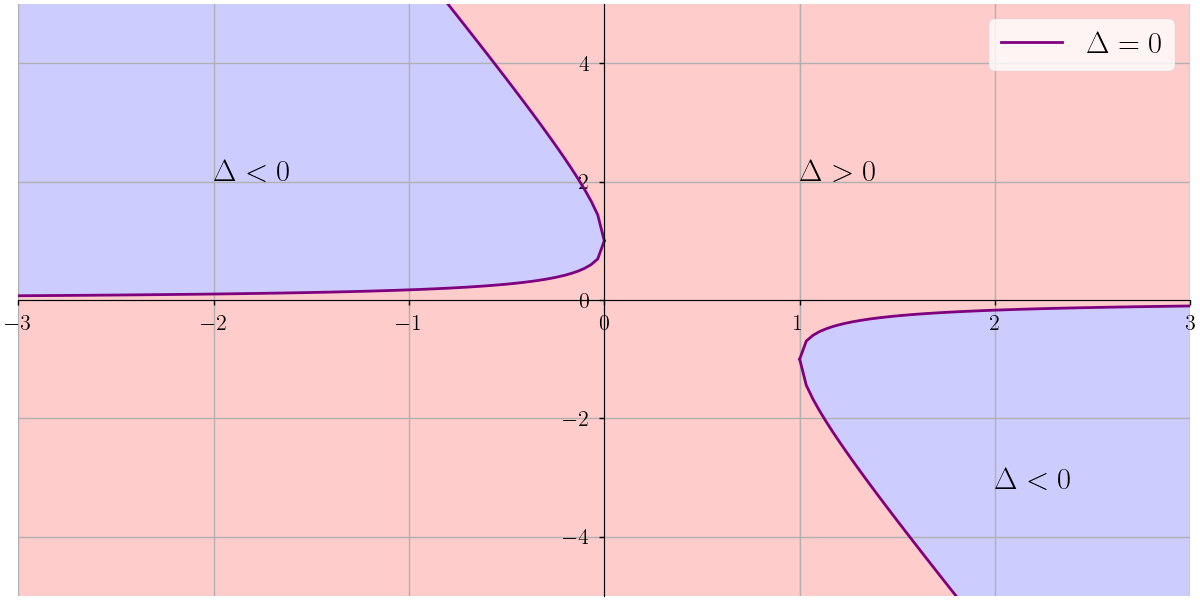
\includegraphics[width=0.5\textwidth]{DeltaDomain}
    \caption{Signe de $\Delta$ en fonction de $\rho$ en abscisses et de $\sigma$ en ordonnées}
    \label{fig:signD}
\end{figure}


\subsubsection*{Cas $\Delta > 0$}
Premièrement on détermine les conditions pour que $\Delta$ soit strictement positif.
\begin{prop}
    $\Delta$ est strictement positif pour l'ensemble des paramètre suivant:
    \[
     \left\{(\sigma,\rho)\in \R ^2 : 1-2 \rho - \sqrt{\frac{(4\rho-2)^2}{4} -1 } > \sigma\ et \ \sigma > 1-2 \rho + \sqrt{ \frac{(4\rho-2)^2}{4} -1  } \right\}    
    \]
\end{prop}

\begin{proof}
    $\Delta = \sigma^2 + \sigma(4\rho-2) + 1$ est un polynome de la variable $\sigma$. On note le deteterminant de $\Delta$ selon la variable $\sigma$, $\delta$. $\Delta$ est convexe par rapport à la variable $\sigma$ donc $\Delta$ est strictement positif à l'éxtérieur de ces racines. On a donc:
    \begin{align*}
        \sigma <& 1-2 \rho - \sqrt{\frac{(4\rho-2)^2}{4} -1 }\\
        \text{ou}\\
        \sigma >& 1-2 \rho + \sqrt{\frac{(4\rho-2)^2}{4} -1 }
    \end{align*}
    %finir demo !
\end{proof}

A présent regardons l'équilibre $0_{\R^3}$ dans le cas $\Delta> 0$
\begin{prop}
    Dans le cas $\Delta>0$ si $\beta<0$ l'équilbre $0_{\R^3}$ est instable, si $\beta >0$ on a :
    \begin{itemize}
        \item Si $\sigma(\rho-1)>0$ alors $0_{\R^3}$ est un equilibre instable pour \eqref{Lorenz}
        \item Si $\sigma(\rho-1)<0$ alors $0_{\R^3}$ est un equilibre assymptotiquement stable pour \eqref{Lorenz}
    \end{itemize}
\end{prop}

\begin{proof}
    Dans le cas $\Delta>0$ on peut expliciter les racines de $\chi$ qui constitue le spectre de la differentielle de $\Gamma$.On a ainsi:
    \[
      \mathrm{Sp}(\mathcal{D}_\Gamma)= \left\{-\beta,\lambda_+ := \frac{-(\sigma+1) + \sqrt{\Delta}}{2},\lambda_- := \frac{-(\sigma+1) - \sqrt{\Delta}}{2}\right\}  
    \]
    Premièrement on différencie le cas $\beta<0$, dans ce cas alors $\max(\mathrm{Sp}(\mathcal{D}_\Gamma))\ge -\beta > 0$, donc dans ce cas $0_{\R^3}$ est un équilibre instable pour \eqref{Lorenz}. Dans le cas où $\beta$ est positif,comme $\lambda_+>\lambda_-$ si $\lambda_+ > 0$ l'équilbre est instable sinon l'équilibre est instable. On cherche alors $\rho$ et $\sigma$ tel que $\lambda_+>0$
    \begin{align*}
        && \frac{-(\sigma+1) + \sqrt{(\sigma-1)^2+4\rho\sigma}}{2} &>0 \\
        \Leftrightarrow && (\sigma-1)^2+4\rho\sigma &> (\sigma+1)^2 \\
        \Leftrightarrow && \sigma(\rho-1) &> 0
    \end{align*}
\end{proof}

\begin{example} 
    Dans cette configuration (figure \ref{fig:EqINS-Dsup0}) on retombe sur les paramètre qui permettent d'observer la trajectoire en forme d'ailes de papillon décrite par E. Lorenz lors de son article de 1963\cite{lorenz1963}. La figure observé apparait pour les paramètres $(\sigma,\rho,\beta) = (10,28,8/3)$. D'après la proposition qui précède c'est donc un cas d'équilibre instable avec $\Delta>0$.

    \begin{figure}[!ht]
        \centering
        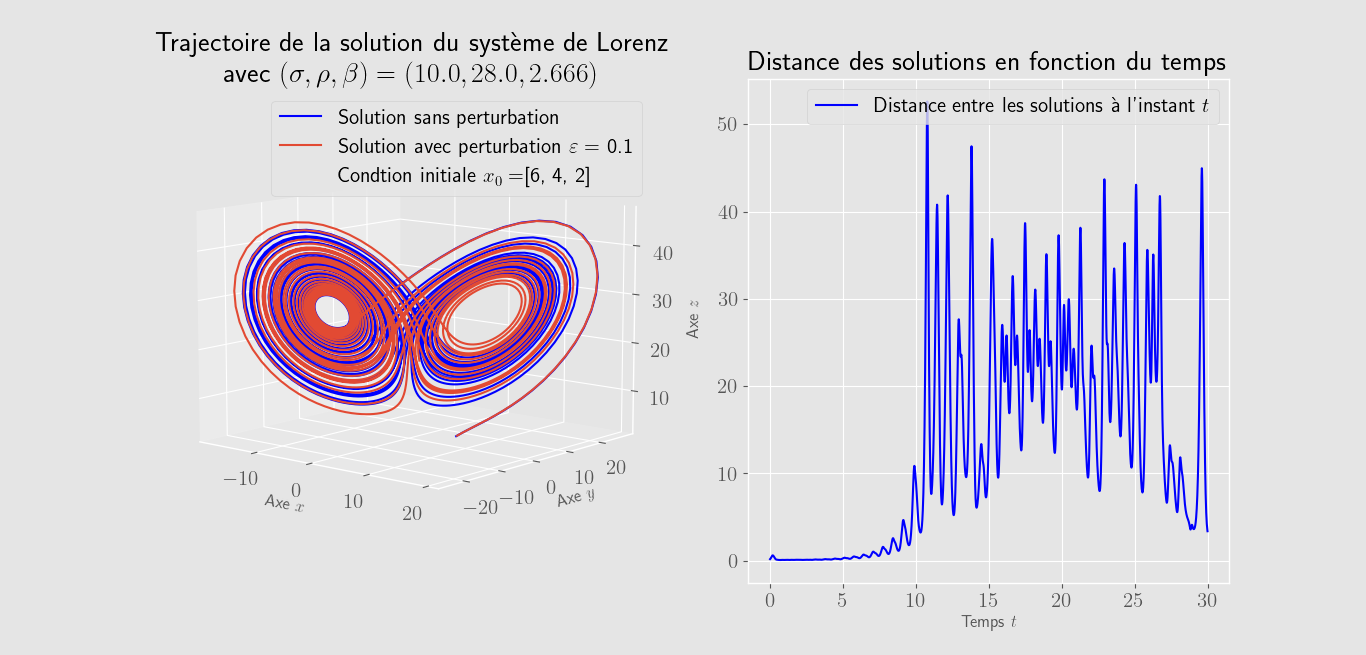
\includegraphics[width = \textwidth]{EqINS-Dsup0}
        \caption{Example d'équilbre instable pour $\Delta>0$}
        \label{fig:EqINS-Dsup0}
    \end{figure}

    Dans la figure \ref{fig:EqAS-Dsup0},on observe bien que les solutions commencent leurs trajectoires avec une distance l'une de l'autre et ensuite se raprochent jusqu'a un ecart très faible. Dans ce cas de figure il est possible de représenter les cas instable, ce qui ne seras pas le cas pour les prochains $\Delta \le 0$.
    
    \begin{figure}[!ht]
        \centering
        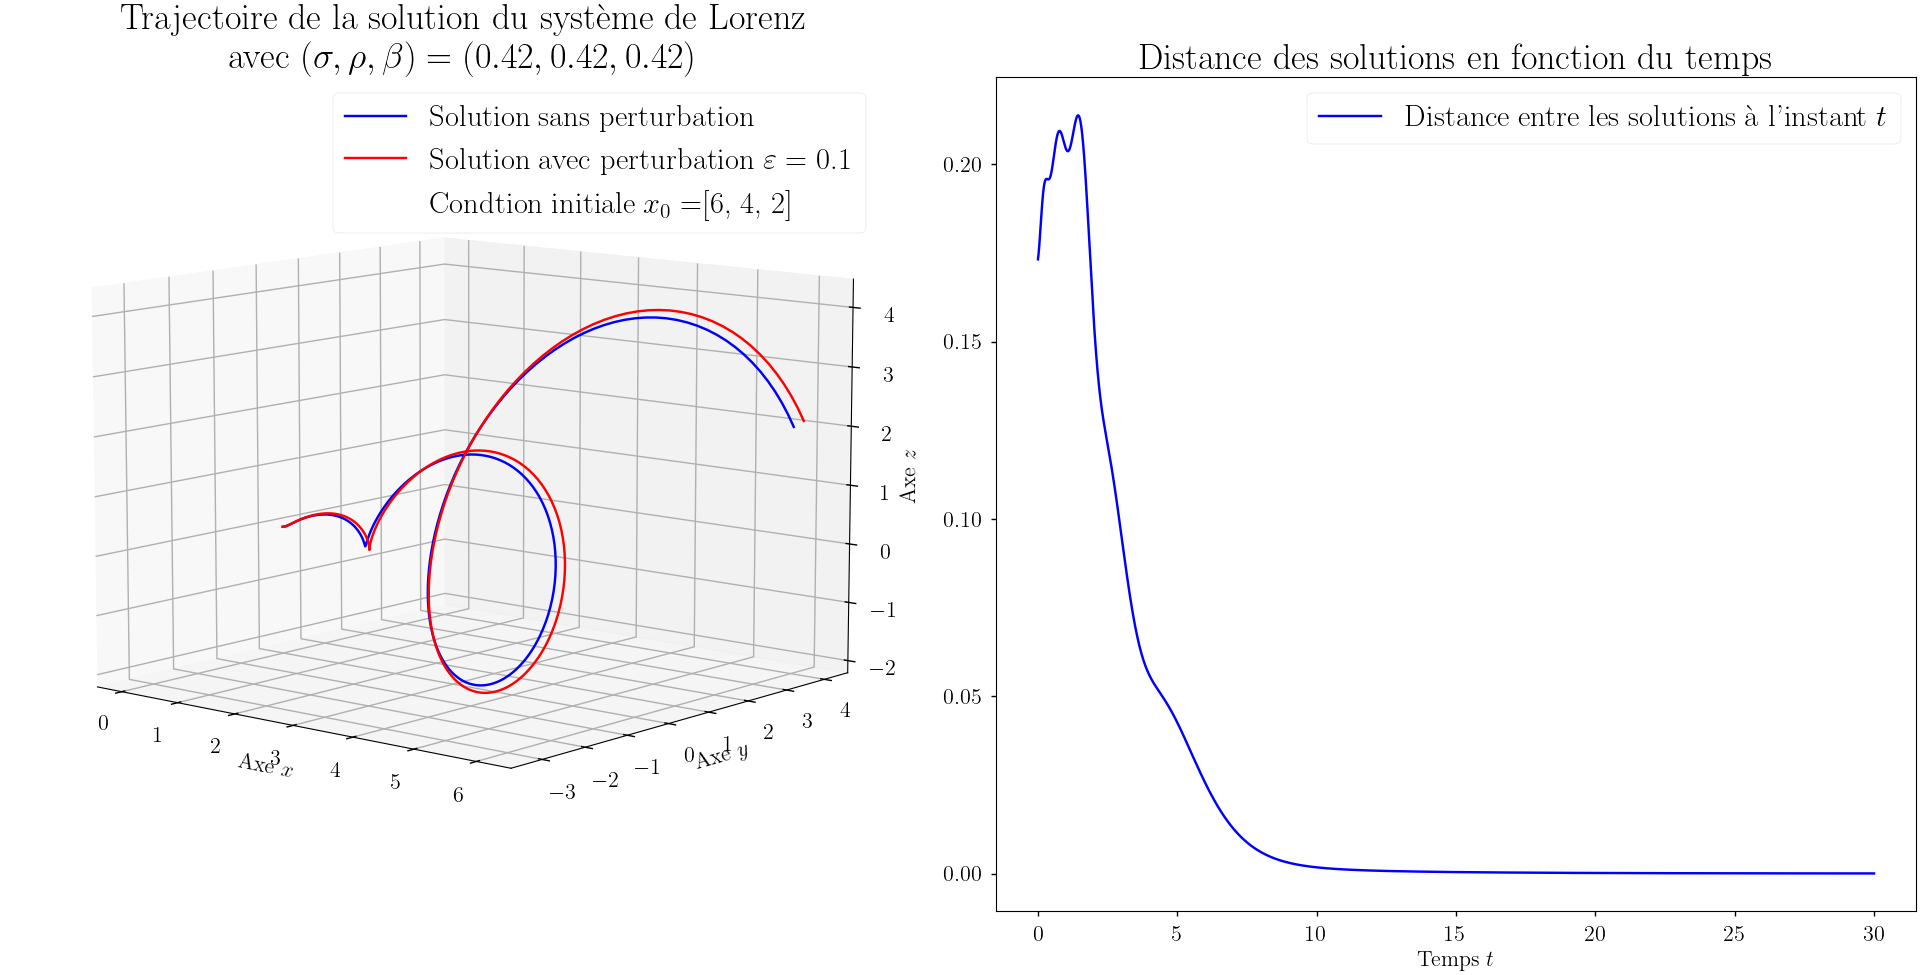
\includegraphics[width = \textwidth]{EqAS-Dsup0}
        \caption{Example d'équilibre assymptotiquement stable pour $\Delta>0$}
        \label{fig:EqAS-Dsup0}
    \end{figure}
    
\end{example}

\subsubsection*{Cas $\Delta = 0$}
On s'intéresse maintenant aux cas tels que $\Delta=0$

\begin{prop} 
    \label{prop:Deg0}
    $\Delta$ est nul si et seulemment si on a la paramétrisation suivante,
    \[
        \left\{(\sigma,\rho)\in \R ^2 :\sigma = 1-2 \rho + \sqrt{ \frac{(4\rho-2)^2}{4} -1 }\ ou\ \sigma = 1-2 \rho - \sqrt{ \frac{(4\rho-2)^2}{4} -1 } \right\}  
    \]
\end{prop}

\begin{example}[Remarque]
    Cette paramétrisation implique que $\rho \in \R \setminus ]0,1[$ 
\end{example}

\begin{proof}
    A nouveaux on considère $\Delta$ comme un polynome de la variable $\sigma$. Pour que $\Delta$ ait des racines il faut que $\delta$ soit positif ou nul.
    \[
    \delta \ge 0 \Leftrightarrow \rho(\rho-1) \ge 0 \Leftrightarrow \rho \in \R \setminus ]0,1[
    \] Maintenant on calcule les racines de $\Delta$.
    \begin{align*}
        \sigma &= \frac{2-4\rho + \sqrt{ (4\rho-2)^2 -4 }}{2} = 1-2 \rho + \sqrt{ \frac{(4\rho-2)^2}{4} -1 }\\
        \text{ou}\\
        \sigma &= \frac{2-4\rho - \sqrt{ (4\rho-2)^2 -4 }}{2} = 1-2 \rho - \sqrt{ \frac{(4\rho-2)^2}{4} -1 }
    \end{align*}
    On obtient ainsi la paramétrisation voulue.
\end{proof}
Maintenant on s'intéresse à la stabilité de l'équilibre pour le cas $\Delta=0$.
% Stabilité pour \Delta = 0
\begin{prop}\label{prop:eqDeg0}
    Dans le cas $\Delta=0$:
    Si $\beta <0$ l'équilbre est instable si $\beta>0$ alors on a:
    \begin{itemize}
        \item Si $\sigma < -1 , \rho > 1$ alors $0_{\R^3}$ est un equilibre instable pour \eqref{Lorenz}
        \item Si $\sigma > -1 , \rho < 1$ alors $0_{\R^3}$ est un equilibre assymptotiquement stable pour \eqref{Lorenz}
    \end{itemize}
\end{prop}
\begin{proof} %DEMO
    Comme $-\beta$ est toujours racine de $\chi$ si $\beta <0$ alors $\max (\mathrm{Sp}(\mathcal{D}_\Gamma)) \ge -\beta > 0$ donc d'après le theoreme \ref{thm:eq-instable}, $0_{\R^3}$ est un équilbre instable pour \eqref{Lorenz}\\
    Si $\beta > 0$ alors dans le cas de $\Delta = 0, \mathrm{Sp}(\mathcal{D}_\Gamma) = \{\beta, -\frac{\sigma+1}{2}\}$, on cherche alors les conditions sur les paramètre $\sigma$ et $\rho$ telles que le système soit instable ou assymptotiquement stable.
    On s'intéresse au cas instable et on inversera le sens des inégalités pour avoir le cas assymptotiquement stable. 
    \[
        -\frac{\sigma+1}{2} >0 \Leftrightarrow \sigma < -1   
    \]
    Dans la première équation on obtient que $-1 > 1-2 \rho + \sqrt{ \frac{(4\rho-2)^2}{4} -1}$ n'as pas de solutions.
    Dans la seconde équation on cherche $\rho$ tel que:
    \[
        1-2 \rho - \sqrt{ \frac{(4\rho-2)^2}{4} -1 } < -1 \Rightarrow \frac{(4\rho-2)^2}{4} -1 > (2\rho-2)^2 \Leftrightarrow \rho > 1 
    \]En faisant les caluls avec l'inégalités inverse on retrouve le cas assymptotiquement stable.
\end{proof}
\begin{example}
    Dans la figure \ref{fig:EqAS-Deg0}n observe bien que les solutions commencent leurs trajectoires avec une distance l'une de l'autre et ensuite se raprochent jusqu'a un ecart très faible. Dans ce cas de figure il n'est pas intéressant de représenter le cas où l'équilibre est instable, car les solutions s'éloignent très rapidement de l'origine et entres elles.
    \begin{figure}[ht]
        \label{fig:EqAS-Deg0}
        \centering
        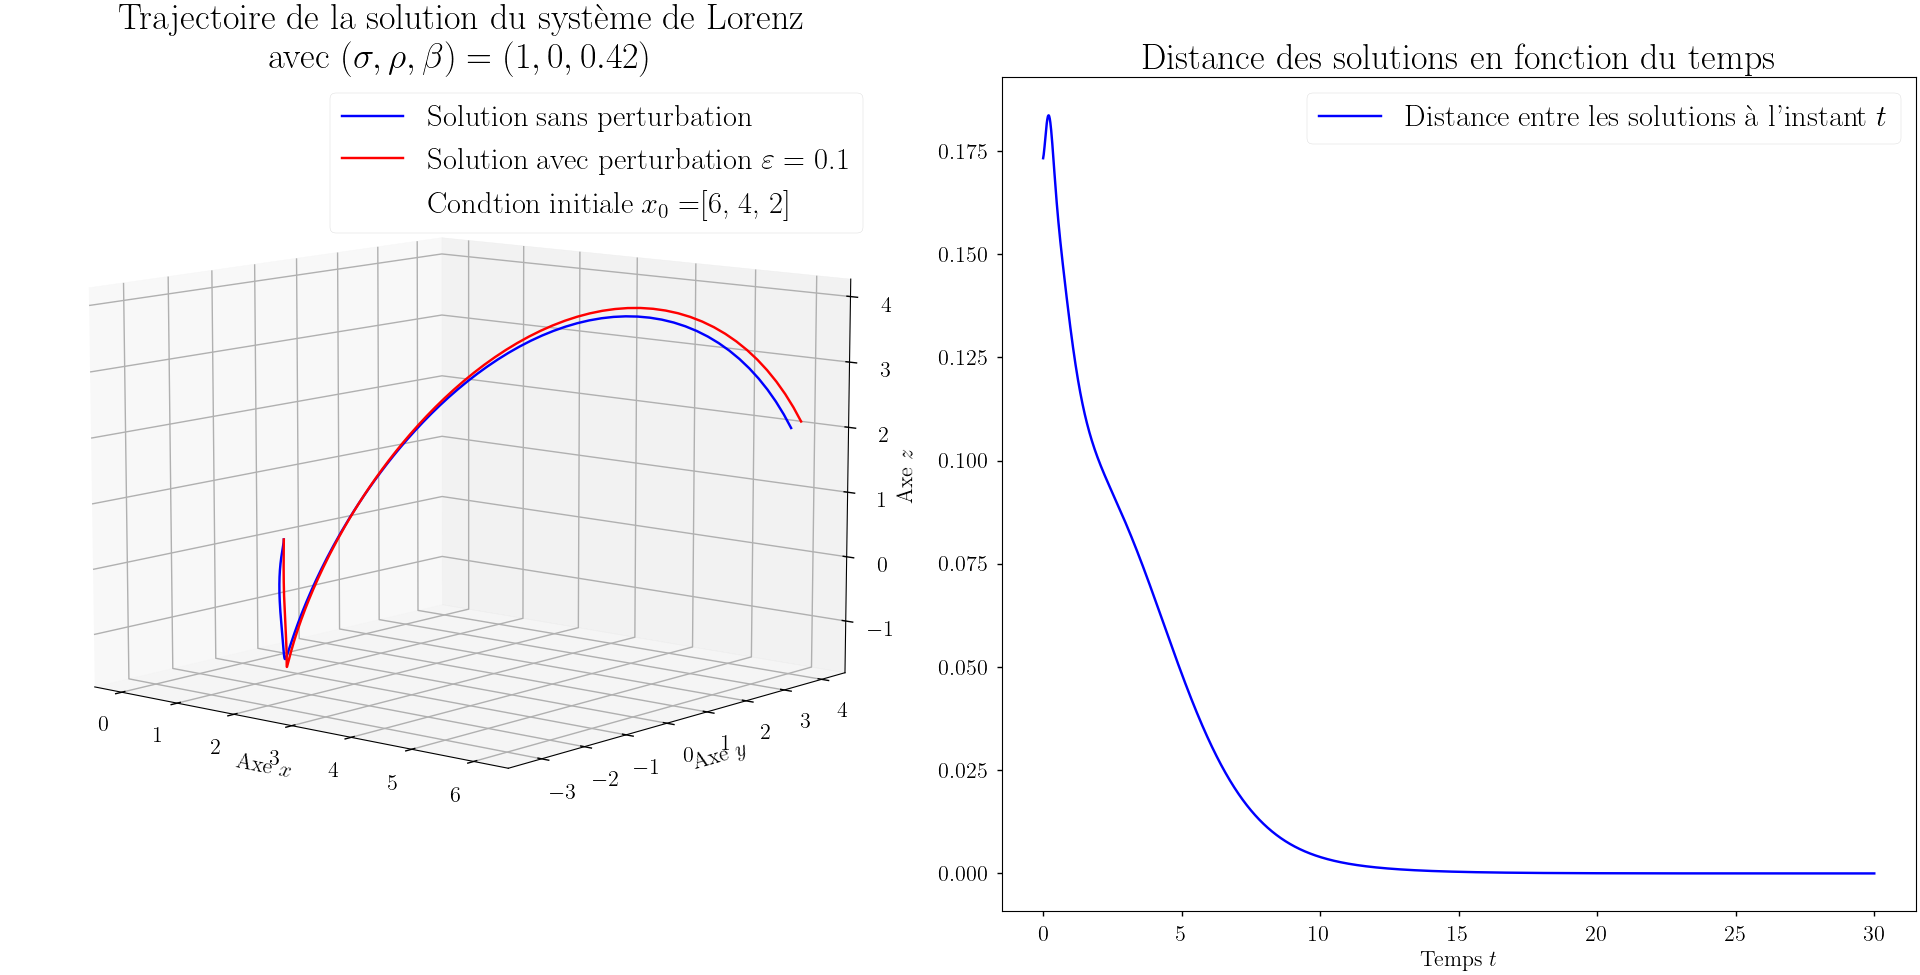
\includegraphics[width = \textwidth]{EqAS-Deg0}
        \caption{Example d'équilibre assymptotiquement stable pour $\Delta=0$}
    \end{figure}
\end{example}

\subsubsection*{Cas $\Delta < 0$}
On determine les cas tels que $\Delta<0$
%CAS \Delta < 0
\begin{prop}
    $\Delta$ est strictement négatif pour l'ensemble des paramètre suivant:
    \[
     \left\{(\sigma,\rho)\in \R ^2 : 1-2 \rho - \sqrt{ \frac{(4\rho-2)^2}{4} -1 }< \sigma < 1-2 \rho + \sqrt{ \frac{(4\rho-2)^2}{4} -1 } \right\}    
    \]
\end{prop}
\begin{example}[Remarque]
    Dans cet ensemble on a que: $\rho \in \R \setminus [0,1]$ 
\end{example}

\begin{proof}
    Pour que $\Delta$ ait des racines il faut que $\delta$ soit strictement positif.
    \[
    \delta > 0 \Leftrightarrow \rho(\rho-1) > 0 \Leftrightarrow \rho \in \R \setminus [0,1]
    \]Par convexité de $\Delta$ on a que $\Delta$ est négatif entre ces racines, il vient alors:
    \[
        1-2 \rho - \sqrt{ \frac{(4\rho-2)^2}{4} -1 } < \sigma < 1-2 \rho - \sqrt{ \frac{(4\rho-2)^2}{4} -1 }
    \]Donc l'ensemble des $\rho,\sigma$ qui verifie cette inégalité sont alors des paramètres tels que $\Delta$ est négatif.
\end{proof}
On determine les cas pour lesquels l'equilibre est instable ou assymptotiquement stable.
% Stabilité cas \Delta < 0
\begin{prop}
    Dans le cas $\Delta<0$:
    Si $\beta <0$ l'équilbre est instable si $\beta>0$ alors on a:
    \begin{itemize}
        \item Si $\sigma < -1 , \rho > 1$ alors $0_{\R^3}$ est un equilibre instable pour \eqref{Lorenz}
        \item Si $\sigma > -1 , \rho < 1$ alors $0_{\R^3}$ est un equilibre assymptotiquement stable pour \eqref{Lorenz}
    \end{itemize}
\end{prop}
\begin{proof}
    Pour la différenciation du cas de $\beta$ cf. la démonstration de \ref{prop:eqDeg0}. Dans ce cas on a:
    \[
        \mathrm{Sp}(\mathcal{D}_\Gamma) = \left\{\beta, \omega := \frac{-(\sigma+1)+ i \sqrt{-\Delta}}{2}, \bar{\omega} := \frac{-(\sigma+1)- i \sqrt{-\Delta}}{2}\right\}
    \]Pour étudier la stabilité on s'intéresse à la partie réelle de $\omega$ et $\bar{\omega}$. Or $\Re (\omega) = \Re (\bar{\omega}) = -\frac{\sigma+1}{2}$ on retombe ainsi sur le même cas que dans la démonstration de la propriété \ref{prop:eqDeg0}. On retrouve bien le cas voulue.
\end{proof}
\begin{example}
    On observe bien que les solutions commencent leurs trajectoires avec une distance l'une de l'autre et ensuite se raprochent jusqu'a un ecart très faible. Dans ce cas de figure il n'est pas intéressant de représenter le cas où l'équilibre est instable, car les solutions s'éloignent très rapidement de l'origine et entres elles.
    
    \begin{figure}[ht]
        \centering
        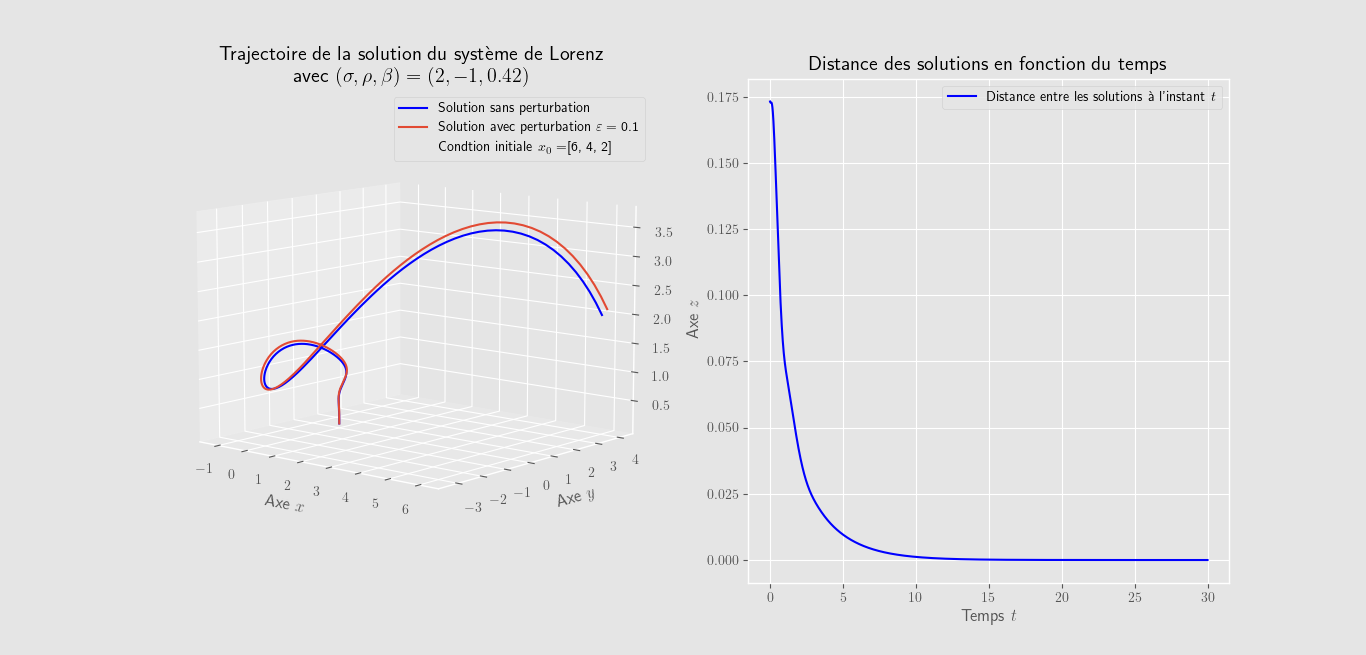
\includegraphics[width = \textwidth]{EqAS-Dinf0}
        \caption{Example d'équilibre assymptotiquement stable pour $\Delta=0$}
    \end{figure}
\end{example}
\subsection{Caractérisation de $S_\pm$}

Dans cette section nous allons nous intéresser au point d'équilibres définit précédemment $S_+$ et $S_-$. Nous ferons aussi quelques hypothèses simplificatrices, supposons $\sigma,\rho,\beta$ positifs et de plus $\sigma>\beta+1$.

\begin{prop}
    Sous les hypothèses de cette section et si $\rho > 1$ alors on definit $\rho^* = \sigma \frac{\sigma+\beta+3}{\sigma-\beta-1}$ tel que 
    \begin{itemize}
        \item si $\rho < \rho^* $ alors les équilibres $S_\pm$ sont assymptotiquement stables pour \eqref{Lorenz}
        \item si $\rho > \rho^* $ alors les équilibres $S_\pm$ sont instables pour \eqref{Lorenz}
    \end{itemize}
\end{prop}

\begin{example}[Remarque]
    Si $\rho \in [0,1]$ les equilibres $S_\pm$ n'existent pas.
\end{example}
\section{Annexes}

\nocite{*}
\printbibliography[heading=bibintoc,title={Bibliographie}]
\end{document}